\documentclass{article}
\usepackage{longtable}
\usepackage{makecell}
\usepackage{float}
\usepackage{graphicx}
\usepackage{bm}
\usepackage{placeins}
\usepackage{threeparttable} 
\usepackage{multirow}
\usepackage{aligned-overset}
\usepackage[slantfont,boldfont]{xeCJK}
\usepackage{fontspec}
\renewcommand{\arraystretch}{1.5}
\setCJKmainfont{SimSun}
\setmainfont{SimSun}
\setsansfont{SimSun}

\title{碰撞实验实验报告}
\author{2411545 邱凯锐}
\date{2025.4.21}

\begin{document}
\maketitle
\section{实验背景}
\hspace*{2em}在经典力学中,碰撞问题是一类传统问题,它在力学基本定律的建立上起过重要作用。碰撞,不仅限于物体间互相接触的冲击作用,物体本身不接触,但相互以力场作用于对方而影响对方的运动状况也称为碰撞。近代关于原子和原子核方面的很多知识,是由观察它们之间的碰撞效应而得知的,使碰撞问题在微观领域获得了新的生命。碰撞问题所涉极为广泛,本实验通过对两个物体对心碰撞的研究,来检验碰撞过程中的动量守恒定律,以及由碰撞而引起的能量改变。 
\section{实验目的}
1. 用对心碰撞特例检验动量守恒定律;\\
2. 了解动量守恒和动能守恒的条件;\\
3. 熟练地使用气垫导轨及数字毫秒计。 
\section{实验原理}
\subsection{验证动量守恒定律}
\hspace*{2em}动量守恒定律指出:若一个物体系所受合外力为零,则物体的总动量保持不变;若物体系所受合外力在某个方向的分量为零,则此物体系的总动量在该方向的分量守恒。\\
\hspace*{2em}设在平直导轨上,两个滑块作对心碰撞,若忽略空气阻力,则在水平方向上就满足动量守恒定律成立的条件,即碰撞前后的总动量保持不变。
\begin{equation}
    m_1u_1+m_2u_2=m_1v_1+m_2v_2
\end{equation}
\hspace*{2em}其中,\(u_1\)、\(u_2\)和\(v_1\)、\(v_2\)分别为滑块\(m_1\)、\(m_2\)在碰撞前后的速度。若分别测出式(1)中各量,且等式左右两边相等,则动量守恒定律得以验证。
\subsection{碰撞后的动量损失}
\hspace*{2em}只要满足动量守恒定律成立的条件,不论弹性碰撞还是非弹性碰撞,总动量都将守恒。但对动能在碰撞过程中是否守恒,还将与碰撞的性质有关。碰撞的性质通常用恢复系数$e$表达:
\begin{equation}
    e=\frac{v_2-v_1}{u_1-u_2}
\end{equation}
\hspace*{2em}式(2)中,\(v_2 - v_1\)为两物体碰撞后相互分离的相对速度,\(u_1 - u_2\)则为碰撞前彼此接近的相对速度。\\
\hspace*{2em}(1) 若相互碰撞的物体为弹性材料,碰撞后物体的形变得以完全恢复,则物体系的总动能不变,碰撞后两物体的相对速度等于碰撞前两物体的相对速度,即\(v_2 - v_1 = u_1 - u_2\),于是\(e = 1\),这类碰撞称为完全弹性碰撞。\\
\hspace*{2em}(2) 若碰撞物体具有一定的塑性,碰撞后尚有部分形变残留,则物体系的总动能有所损耗,转变为其它形式的能量,碰撞后两物体的相对速度小于碰撞前的相对速度,即\(0 < v_2 - v_1 < u_1 - u_2\)于是,\(0 < e < 1\),这类碰撞称为非弹性碰撞。\\
\hspace*{2em}(3) 碰撞后两物体的相对速度为零,即\(v_2 - v_1 = 0\)或\(v_2 = v_1 \equiv v\),两物体粘在一起以后以相同速度继续运动,此时\(e = 0\),物体系的总动能损失最大,这类碰撞称为完全非弹性碰撞,它是非弹性碰撞的一种特殊情况。\\
\hspace*{2em}三类碰撞过程中总动量均守恒,但总动能却有不同情况。由式(1)和(2)可求碰撞后的动能损失\(\Delta E_{k}=\frac{1}{2}m_{1}m_{2}(1 - e^{2})(u_{1}-u_{2})^{2}/(m_{1}+m_{2})\)。①对于完全弹性碰撞,因\(e = 1\),故\(\Delta E_{k}=0\),即无动能损失,或称动能守恒。②对于完全非弹性碰撞,因\(e = 0\),故:\(\Delta E_{k}\equiv\Delta E_{kM}\),即动能损失最大。③对于非完全弹性碰撞,因\(0 < e < 1\),故动能损失介于二者之间,即:\(0 < \Delta E_{k}<\Delta E_{kM}\)。 
\subsection{\(m_1 = m_2 \equiv m\),且\(u_2 = 0\)的特定条件下,两滑块的对心碰撞。}
(1)对完全弹性碰撞,\(e = 1\),式(1)和(2)的解为\\
\begin{equation}
    \left.\begin{array}{l}
    v_1 = 0 \\
    v_2 = u_1
    \end{array}\right\}
\end{equation}
由式(3)可知,当两滑块质量相等,且第二滑块处于静止时,发生完全弹性碰撞的结果,使第一滑块静止下来,而第二滑块完全具有第一滑块碰撞前的速度,“接力式”地向前运动。若式(3)得到验证,则说明完全弹性碰撞过程中动量守恒,且$e = 1$,$\Delta E_{k}=0$,即动能亦守恒。\\
\hspace*{2em}以上讨论是理想化的模型。若两滑块质量不严格相等、两挡光物的有效遮光宽度$\Delta s_1$及$\Delta s_2$也不严格相等,则碰撞前后的动量百分差$E_1$为:
\begin{equation}
    E_1=\frac{|P_2 - P_1|}{P_1}=\left|\frac{m_2\Delta s_2\Delta t_1}{m_1\Delta s_1\Delta t_2}-1\right|
\end{equation}
动能百分差$E_2$为:
\begin{equation}
    E_2=\frac{|E_{k2}-E_{k1}|}{E_{k1}}=\left|\frac{m_2\Delta s_2^{2}\Delta t_1^{2}}{m_1\Delta s_1^{2}\Delta t_2^{2}} - 1\right|
\end{equation}
若$E_1$及$E_2$在其实验误差范围之内,则说明上述结论成立。\\
(2)对于完全非弹性碰撞,式(1)和(2)的解为:\\
\begin{equation}
    v_1 = v_2 \equiv v = \frac{u_1}{2}
\end{equation}
若式(6)得证,则说明完全非弹性碰撞动量守恒,且$e = 0$,其动能损失最大,约为50\%。\\
\hspace*{2em}考虑到完全非弹性碰撞时可采用同一挡光物遮光,即有:$\Delta s_2' \equiv \Delta s_1'$。同样可求得其动量和动能百分差$E_1'$及$E_2'$分别为:
\begin{equation}
    E_1'=\frac{|P_2' - P_1'|}{P_1'}=\left|\left(1 + \frac{m_2}{m_1}\right)\frac{t_1'}{t_2'} - 1\right|
\end{equation}
\begin{equation}
    E_2'=\frac{|E_{k2}' - E_{k1}'|}{E_{k1}'}=\left|\left(1 + \frac{m_2}{m_1}\right)\left(\frac{\Delta t_1'}{\Delta t_2'}\right)^2 - 1\right|
\end{equation}
显然,其动能损失的百分误差则为:
\begin{equation}
    E_{\Delta}=\left|2\left(1 + \frac{m_2}{m_1}\right)\left(\frac{\Delta t_1'}{\Delta t_2'}\right)^2 - 1\right|
\end{equation}
若$E_1'$及$E_{\Delta}$在其实验误差范围内,则说明上述结论成立。
\section{实验仪器}
\hspace*{2em}仪器用品包括:气垫导轨及附件(如图 所示,包括滑块及挡光框各一对)、数字毫秒计、物理天平及游标卡尺等。 
\begin{figure}[!h]
    \centering
    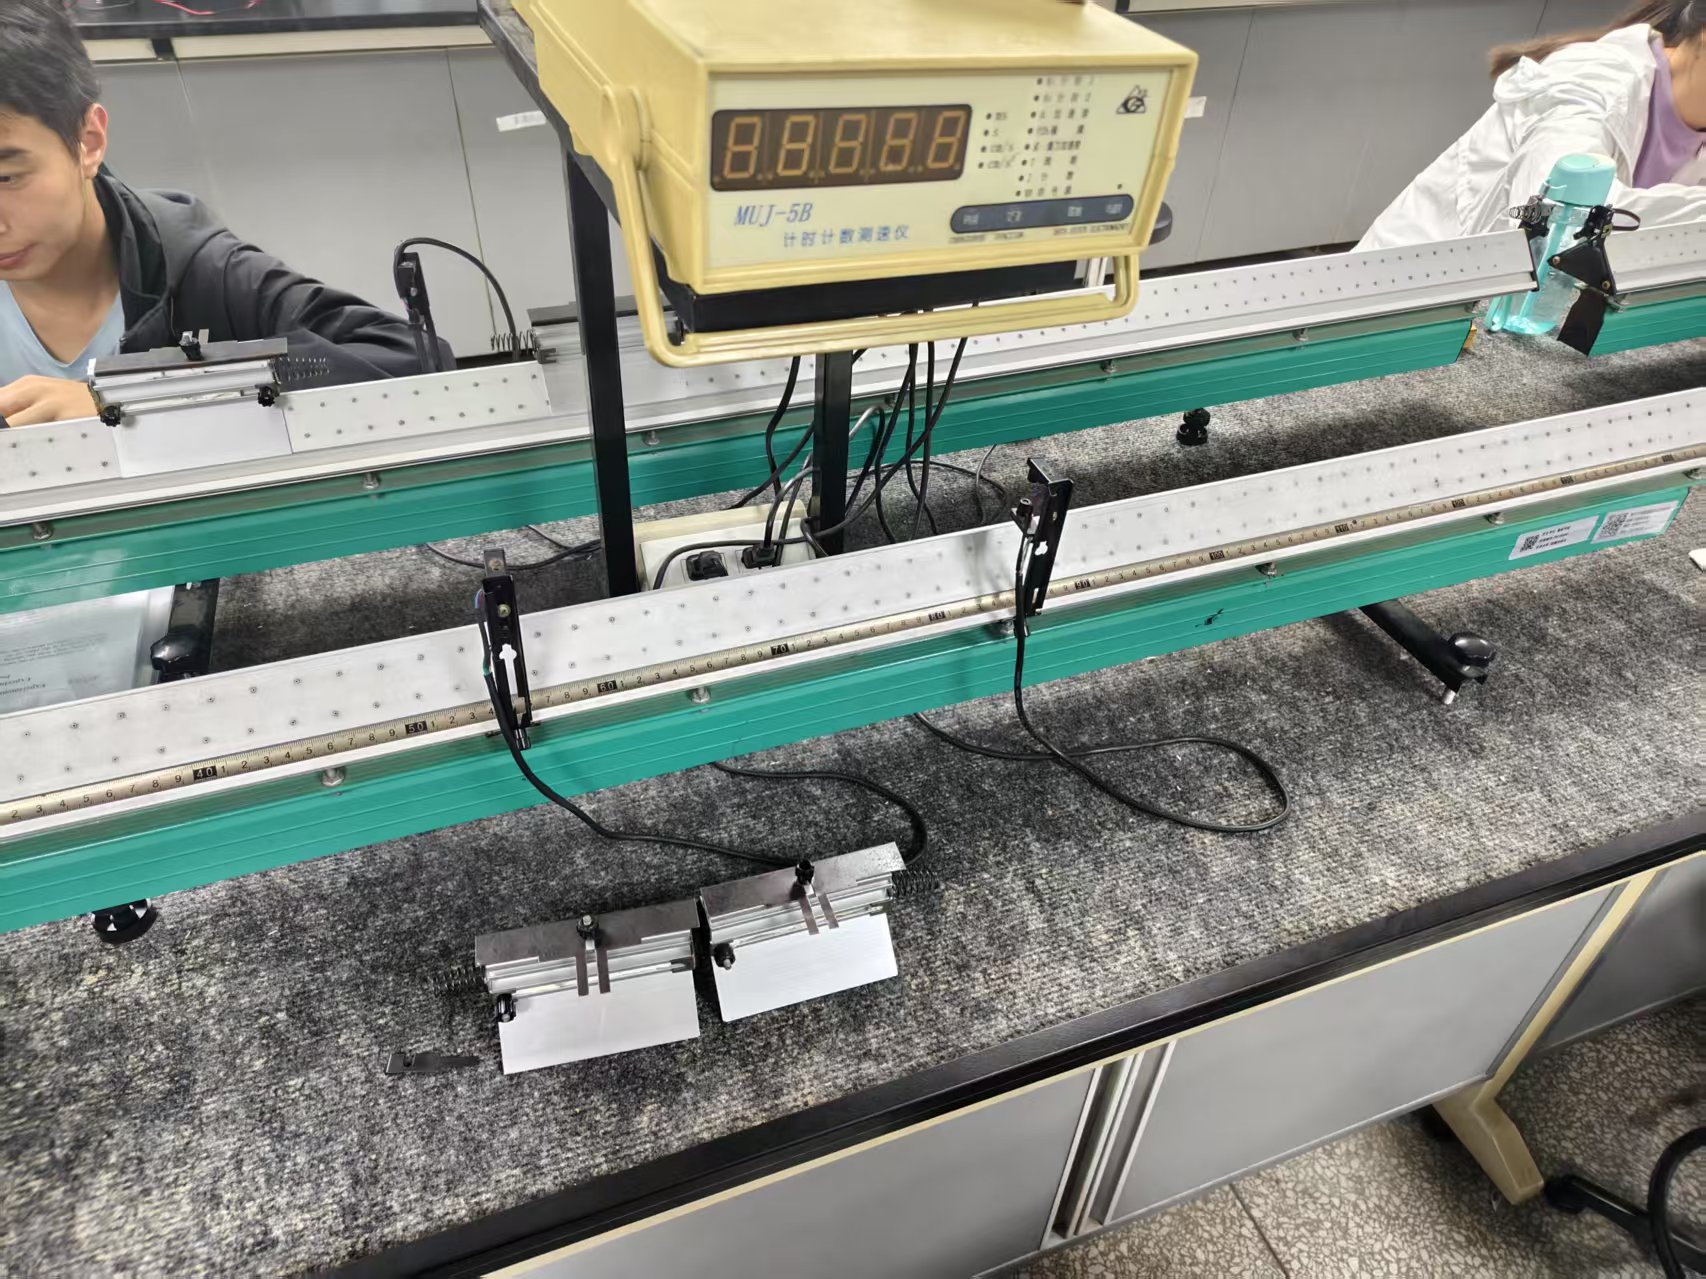
\includegraphics[width=8cm]{1.jpg}
\end{figure}
\section{实验内容}
\hspace*{2em}1. 用动态法调平导轨,使滑块在选定的运动方向上作匀速运动,以保证碰撞时合外力为零的条件;\\
\hspace*{2em}2. 用物理天平校验两滑块(连同挡光物)的质量\(m_1\)及\(m_2\);\\
\hspace*{2em}3. 用游标卡尺测出两挡光物的有效遮光宽度\(\Delta s_1\)、\(\Delta s_2\)及\(\Delta s_1'\);\\
\hspace*{2em}4. 在\(m_1 \approx m_2 \equiv m\)的条件下,测完全弹性和完全非弹性碰撞前后两滑块各自通过光电门一及二的时间\(\Delta t_1\)、\(\Delta t_2\)及\(\Delta t_1'\)、\(\Delta t_2'\)。
\section{实验数据与结论}
\subsection{滑块参数}
\hspace*{2em}调平导轨后,测量滑块1、2的相关参数。
\begin{table}[ht]
    \centering
    \begin{tabular}{lllll}
    \hline\hline
      & m/g & $\Delta s_1/\mathbf{cm}$ & $\Delta s_2/\mathbf{cm}$ & $\Delta s_1'/\mathbf{cm}$ \\
    滑块1 & 129.80  &  0.550  &  1.590  &  1.040 \\
    滑块2 & 129.80  &  0.552  &  1.570  &  1.018 \\
    \hline\hline  
    \end{tabular}
    \end{table}
\subsection{完全弹性碰撞}
\hspace*{2em}改变滑块的初始速度,记录碰前和碰后滑块通过光电门的时间$\Delta t_1、\Delta t_2$,并计算对应的碰前速度$u$和碰后速度$v$,以及恢复系数e,动量百分差$E_1$和动能百分差$E_2$。\\
\begin{table}[ht]
    \centering
    \begin{tabular}{ccc|ccccc}
    \hline\hline
    \multirow{2}{*}{组别} & \multicolumn{2}{c}{碰前} & \multicolumn{2}{c}{碰后} & \multirow{2}{*}{e} & \multirow{2}{*}{$E_1$} & \multirow{2}{*}{$E_2$} \\
                        & $\Delta t_1$(ms)      & u(m/s)            & $\Delta t_2$(ms)      & v(m/s)            &                    &                     &                     \\
    1                   & 23.31   & 0.4461  & 24.18   & 0.4210   & 0.9436        & 0.056         & 0.11         \\
    2                   & 21.21   & 0.4903  & 21.87   & 0.4654  & 0.9493        & 0.051         & 0.099          \\
    3                   & 28.04   & 0.3708  & 28.87   & 0.3526  & 0.9507        & 0.049         & 0.096        \\
    \hline\hline
    \end{tabular}
\end{table}
\hspace*{2em}$E_1$和$E_2$在其实验误差范围之内,说明完全弹性碰撞的结论成立。
\subsection{完全非弹性碰撞}
\hspace*{2em}改变滑块的初始速度,记录碰前和碰后滑块通过光电门的时间$\Delta t_1'、\Delta t_2'$,并计算对应的碰前速度$u'$和碰后速度$v'$,以及动量百分差$E_1'$和动能损失百分误差$E_{\Delta}$。\\
\begin{table}[!h]
    \centering
    \begin{tabular}{ccc|cccc}
    \hline\hline
    \multirow{2}{*}{组别} & \multicolumn{2}{c}{碰前} & \multicolumn{2}{c}{碰后} & \multirow{2}{*}{$E_1'$} & \multirow{2}{*}{$E_{\Delta}$} \\
                        & $\Delta t_1'$(ms)      & $u'$(m/s)            & $\Delta t_2'$(ms)      & $v'$(m/s)            &                     &                     \\
                        1                   & 29.93                  & 0.3475           & 59.69                  & 0.1705           & 0.018                            & 0.036                             \\
                        2                   & 26.62                  & 0.3907            & 52.53                  & 0.1938           & 0.0079                             & 0.016                              \\
                        3                   & 24.14                  & 0.4308           & 48.35                  & 0.2105           & 0.023                             & 0.045                            \\
    \hline\hline
    \end{tabular}
\end{table}
\hspace*{2em}$E_1'$和$E_\Delta$在其实验误差范围之内,说明完全非弹性碰撞的结论成立。
\section{思考题}
1.\textbf{完全弹性碰撞的特点是什么?试证明在完全弹性碰撞中,碰撞后两物体分离的速度\(v_2 - v_1\)等于碰撞前两物体相互接近的速度\(u_1 - u_2\)。}\\
\hspace*{2em}完全弹性碰撞的特点是碰撞前后,系统的总动量和总动能不发生改变。下证:$v_2-v_1=u_1-u_2$。\\
\hspace*{2em}根据碰撞前后系统总动量守恒:
\begin{equation}
    m_1u_1+m_2u_2=m_1v_1+m_2v_2
\end{equation}
总动能守恒:
\begin{equation}
    \frac{1}{2}m_1u_1^2+\frac12m_2u_2^2=\frac12m_1v_1^2+\frac12m_2v_2^2
\end{equation}
将式(11)移项后除以式(10),得到:
\begin{equation*}
    u_1+v_1=v_2+u_2
\end{equation*}
即:
\begin{equation}
    v_2-v_1=u_1-u_2
\end{equation}
2.\textbf{设两滑块质量及速度大小均相同,相对碰撞后,两滑块的运动情况将如何?}\\
\hspace*{2em}根据动量守恒
\begin{equation}
    0=mv+m(-v)=mu_1+mu_2
\end{equation}
得到
\begin{equation}
    u_1=-u_2
\end{equation}
(1)发生完全弹性碰撞:$u_1=-u_2=-v$,两物体以原速度大小,朝反向运动;\\
(2)发生非弹性碰撞:$u_1=-u_2=-v',|v'|<|v|$,两物体以$|v'|$的速度,朝反向运动;\\
(3)发生完全非弹性碰撞:$u_1=-u_2=0$,两物体静止。
\end{document}